\documentclass[10pt,journal,compsoc]{IEEEtran}
\usepackage{grffile}
\usepackage[dvips]{graphicx}
\usepackage[cmex10]{amsmath}

\hyphenation{}

\begin{document}

\title{TP de mierda!}


\author{Lucila Stancato,~\IEEEmembership{I.T.B.A,}
		Dami\'an Modernell,~\IEEEmembership{I.T.B.A,}
		Juan Brasca,~\IEEEmembership{I.T.B.A,}
		Conrado Negro,~\IEEEmembership{I.T.B.A}%
}

\IEEEcompsoctitleabstractindextext{%
\begin{abstract}
%\boldmath
Simulamos un modelo de cola simple con un esquema de simulaci\'on forzada por eventospara comparar
los resultados con los valores te\'oricos de dicho modelo. Dise\~namos un modelo de un sistema de
dos colas en serie para hacer simulaciones y obtener una estimaci\'on de los par\'ametros del sistema.
\end{abstract}

\begin{IEEEkeywords}
Teor\'ia de colas, modelo de cola simple, simulaci\'on forzada por eventos
\end{IEEEkeywords}
}%\IEEEcompsoctitleabstractindextext

\maketitle

\IEEEdisplaynotcompsoctitleabstractindextext

\IEEEpeerreviewmaketitle

\section{Introducci\'on}
La teor\'ia de colas fue originada por Agner Krarup Erlang (1878-1929) en 1909. Es una colecci\'on
de modelos matem\'aticos que describen sistemas de l\'ineas de espera (o colas) particulares o de
sistemas de colas. Esta teor\'ia es de gran valor en los negocios de hoy en d\'ia ya que muchos de
sus problemas pueden modelarse como problemas de congesti\'on llegada/partida.\\
El modelo del sistema de una cola puede verse en la figura 1. Consiste en clientes que van a ser
atendidos por un servidor. En el caso de que el servidor este desocupado y llegue un cliente, entonces
este es atendido inmediatamente. Si el servidor estuviera ocupado, entonces el cliente espera en la
cola hasta que el servidor se desocupe.\\

\begin{figure}[t]
\label{fig:colasimple}
\begin{center}
\centering
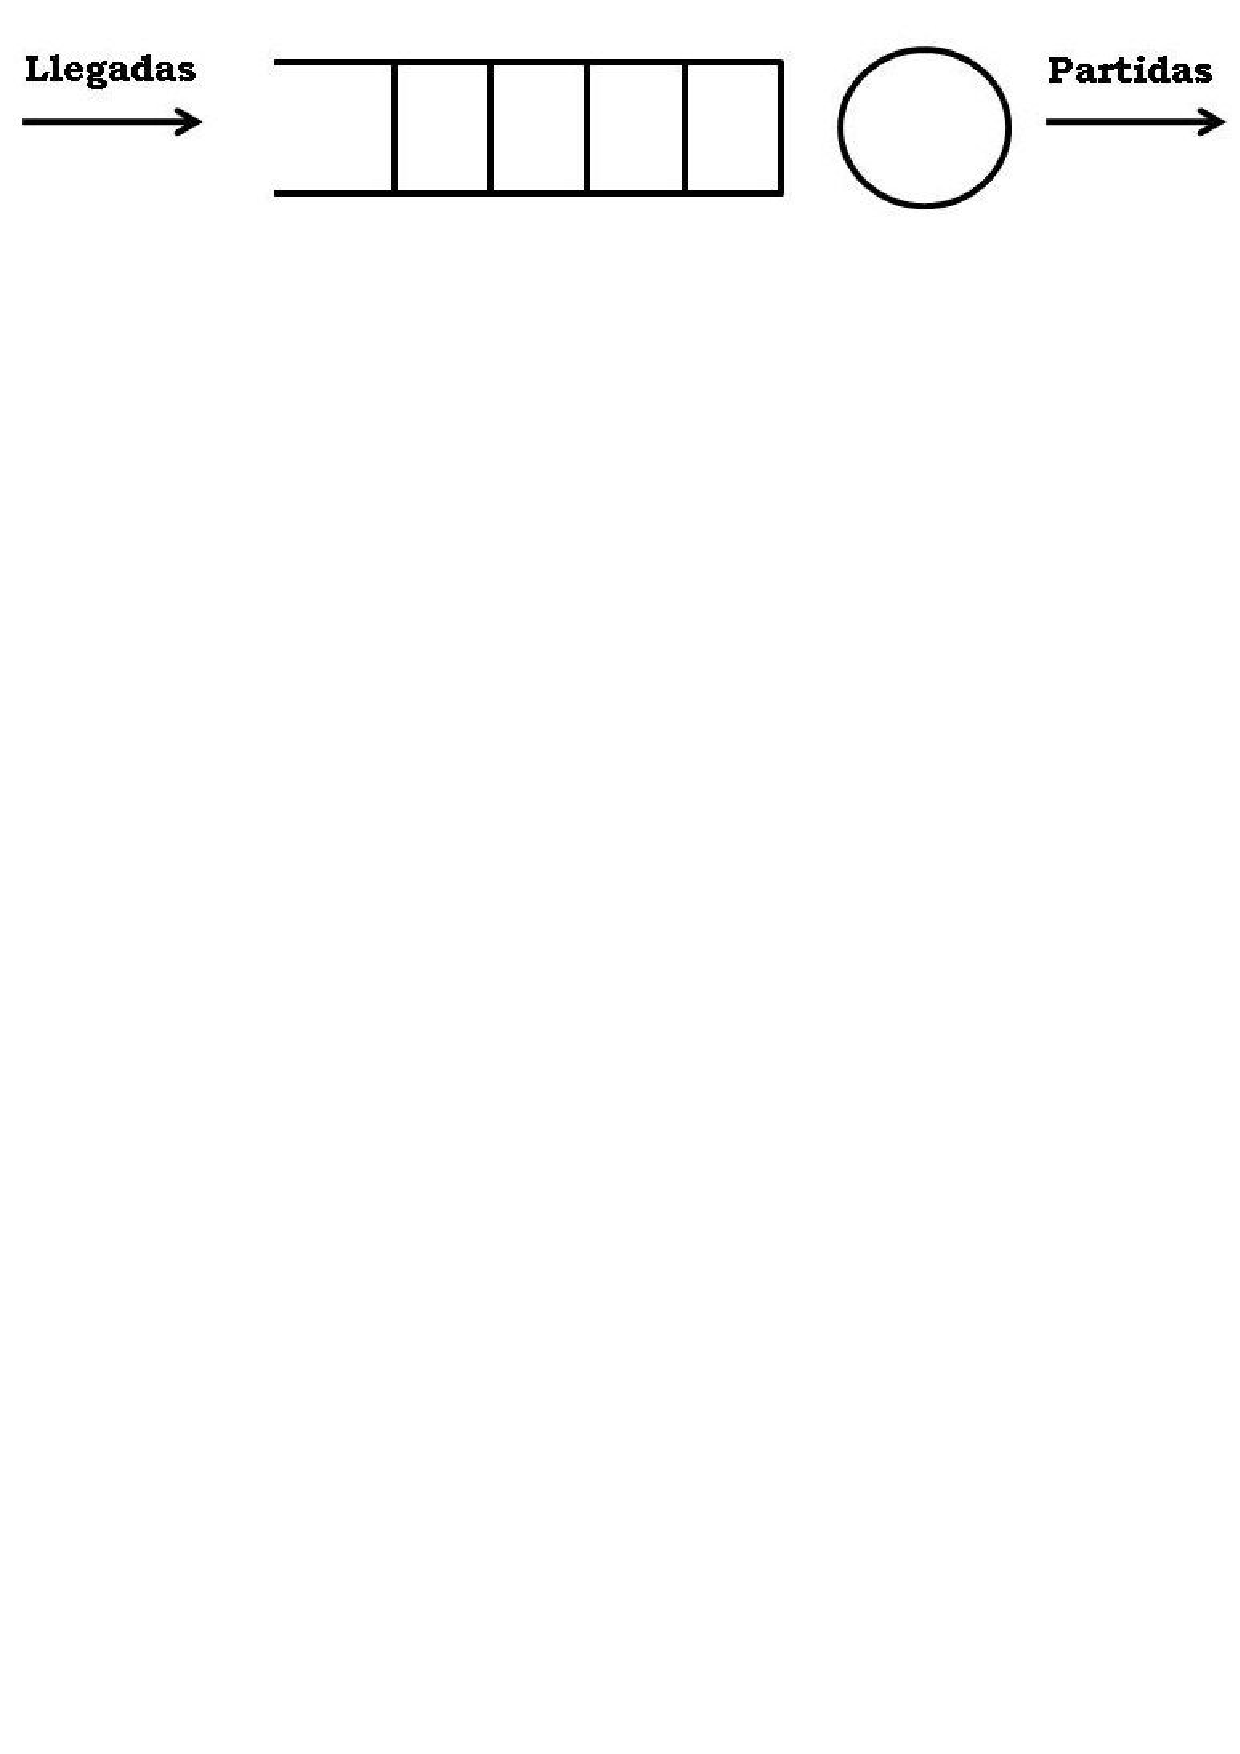
\includegraphics[width=3.2in]{cola.jpg}
\caption{Modelo de cola simple}
\end{center}
\end{figure}

El problema es determinar qu\'e capacidad tiene la cola o qu\'e tasa de servicio tiene el servidor ya
que ni los clientes llegan a tiempos fijos ni los tiempos de servicio son iguales para todos los
clientes. Nosotros utilizamos un modelo de cola simple de tipo M/M/1/$\inf$/FIFO en el que tanto el
tiempo entre arribos de clientes como el tiempo de servicio son variables aleatorias con distribuci\'on
exponencial. Tambi\'en supone que la cola tiene capacidad infinita, y sigue una disciplina de tipo FIFO.\\
Este modelo es el m\'as simple de analizar mediante la simulaci\'on por eventos discretos. La simulaci\'on
forzada por eventos discretos es una t\'ecnica inform\'atica de modelado din\'amico de sistemas. Estos
sistemas se caracterizan por mantener un estado interno global que cambia en instantes de tiempo asociados
a la ocurrencia de un determinado evento en la din\'amica del sistema. En nuestro caso, el conjunto discreto
de eventos del sistema es $E={llegada, partida}$, y el conjunto de estados del servidor es $S={libre, ocupado}$.\\
##########En la secci\'on 2 hacemos ESTOOOOOOO en la seccion 3 hacemos ESTOOOOOOOOOOOOOO blablabla!!##############

%para meter graficos
%-------------------
%\begin{figure}[t]
%\label{fig:histogramalecuyer}
%\begin{center}
%\centering
%\includegraphics[width=3.2in]{clases.jpg}
%\caption{10000 n\'umeros generados con el generador de L'Ecuyer divididos en 10 intervalos de clase que muestran una distribuci\'on uniforme}
%\end{center}
%\end{figure}

%para meter tablas
%-----------------
%\begin{table}[!t]
%\renewcommand{\arraystretch}{1.3}
%\caption{Semillas de las variables pseudoaleatorias}
%\centering
%\begin{tabular}{c c}
%\hline
%\hline
%Variable  & Semilla\\
%\hline
%$u_1$ &  23\\
%$u_2$ & 2 \\
%$u_3$ & 5 \\
%$u_4$ & 17  \\
%$u_5$ & 7 \\
%\hline
%\hline
%\end{tabular}
%\label{tab:sim}
%\end{table}

\section{C\'alculo de par\'ametros del sistema}
Para distintos sistemas como podr\'ia ser la cola de un banco, o de cualquier servicio que pueda ser
simulado por el sistema de colas, puede llegar a ser muy \'util conocer distintos par\'ametros como
por ejemplo el promedio temporal de clientes en el sistema, o el tiempo medio que un cliente tarda
en el sistema.

Estimamos con un error menor al 5\%, el promedio temporal de clientes en el sistema
cuyo valor te\'orico se calcula con la ecuaci\'on 1

\begin{equation}
L = \frac{1}{T} \int_{0}^{T}L(t)dt 
\end{equation}

donde L(T) es la cantidad de clientes en el sistema en el instante t, para un tiempo de operaci�n
de la cola T. Para lograrlo, simulamos la cola mediante una simulaci\'on forzada por eventos realizada
en Matlab y determinamos que se deben realizar XXXXXXXXXXXXXXXXXXX simulaciones para tener un error
menor al 5%.
%chamuyo
En un caso pr\'actico, conocer este par\'ametro puede resultar \'util para saber si es necesario
tener otra cola si la cantidad de clientes en el sistema con una sola cola es demasiado grande.

%%%%%%%%%%%%%%%%%%%%
%poner los resultados teoricos y los estimados, calcular la diferencia y chamuyar
%%%%%%%%%%%%%%%%%%%%


En algunos casos, se puede necesitar conocer el tiempo medio que un cliente tarda en el sistema. 
Siempre se desea que este par\'ametro sea menor para que la atenci\'on a los clientes sea m\'as r\'apida.
Estimamos este tiempo simulando la misma cola que en la secci\'on 1 y tambi\'en con un error menor al 5%.

%%%%%%%%%%%%%%%%%%%%
%poner los resultados teoricos y los estimados, calcular la diferencia y chamuyar
%%%%%%%%%%%%%%%%%%%%

\section{Sistema de dos colas en serie}



\section{Conclusi\'on}


\begin{thebibliography}{1}

\bibitem{IEEEhowto:kopka}
Teor\'ia de colas, http://exa.unne.edu.ar/depar/areas/informatica/evalua/teoria_de_colas.pdf

\bibitem{IEEEhowto:kopka}
Simulaci\'on de eventos discretos, http://es.wikipedia.org/wiki/Simulaci\%C3\%B3n_por_eventos_discretos

\bibitem{IEEEhowto:kopka}


\end{thebibliography}

\end{document}


